\documentclass[../../main.tex]{subfiles}


\begin{document}

\subsection*{(a)}
After selecting the three specified attributes, normalization by Z-transformation is done. The result is multiplied so it can be fed to all k-means clusterers at once. For each clustering we set the necessary 'k' and 'max runs' and select the 'add as label' checkbox so the cluster labels are added as a new column. To use the unscaled dataset we first reverse the Z-transformation by De-Normalizing and then apply it to the clustered data.\\  
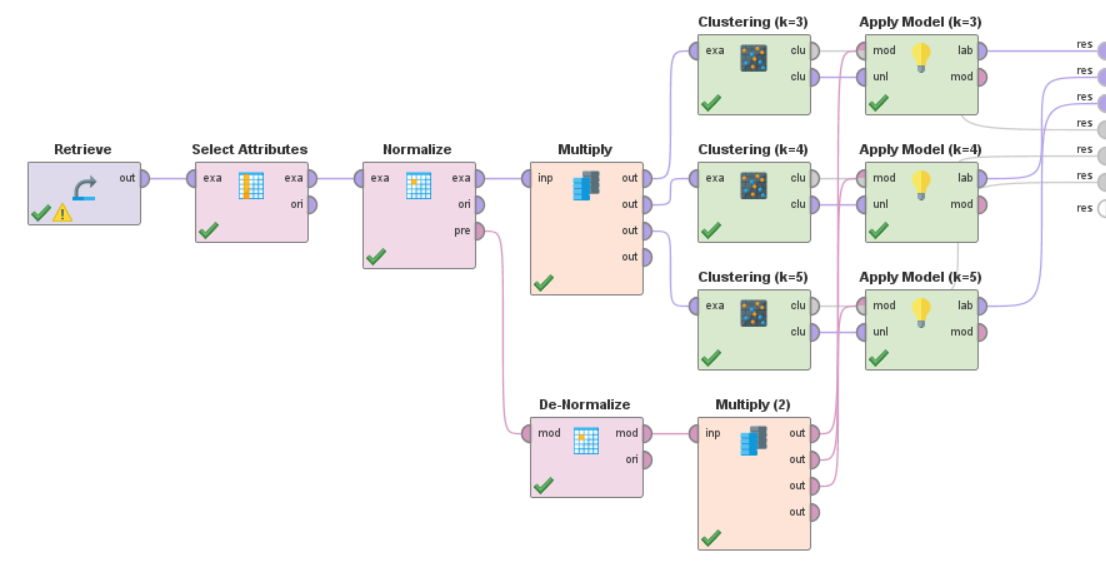
\includegraphics[width=\textwidth]{img/QUESTION_3a_PROCESS.png}

The following graphics show the clustering results for Number of Offers mapped against the Requested Amount. Over all $k\in\{3,4,5\}$ there are a few similar clusters:
\begin{itemize}
\item \texttt{Low Requested Amount (mostly 0-25k) and low Number of Offers (0-2.5)}. However this region is further split with higher k's.
\item \texttt{Higher Requested Amount (mostly >25k) and low Number of Offers (mostly 0-2.5)}. This class is very similar over all k.
\item \texttt{Higher Number of Offers (>2.5)}. Only k=3 also clusters in lower values because of a lack of options.
\end{itemize}
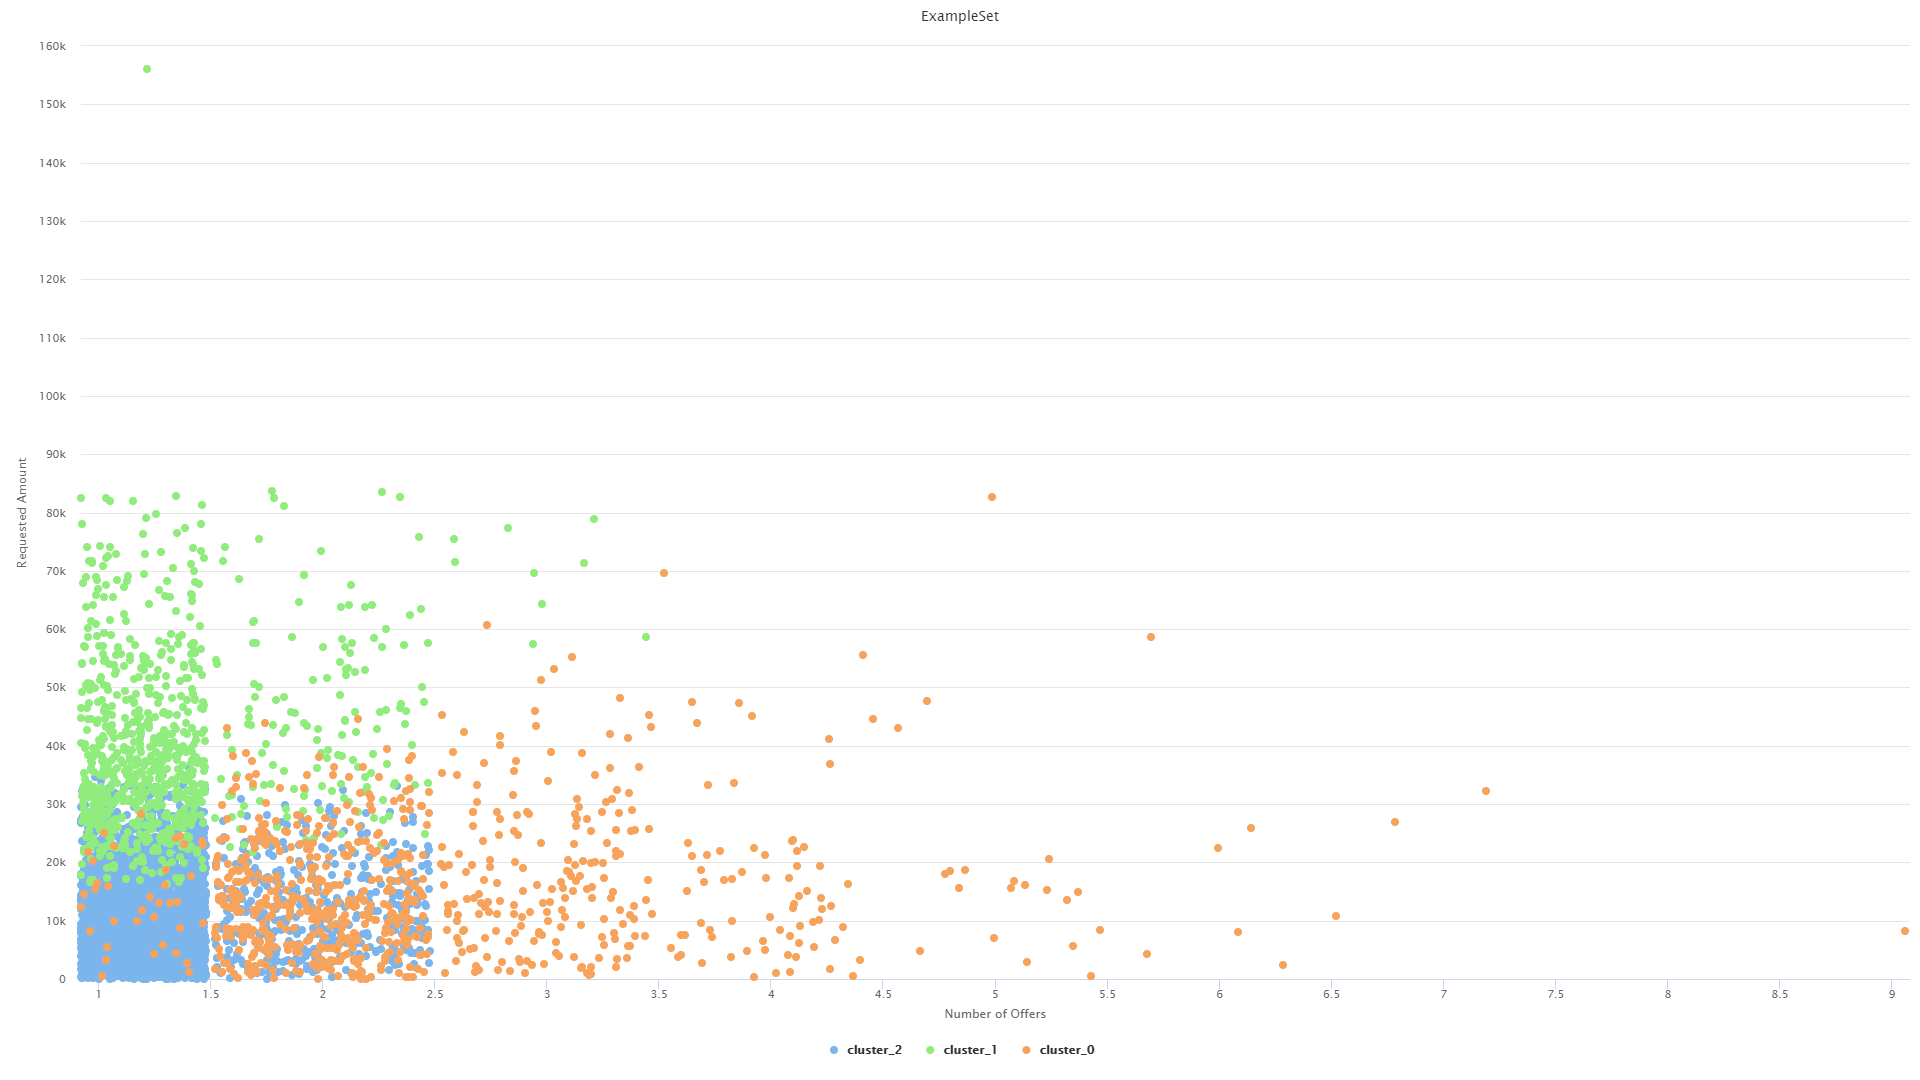
\includegraphics[width=\textwidth]{img/QUESTION_3a_kmeans_3_offers_amount.png}
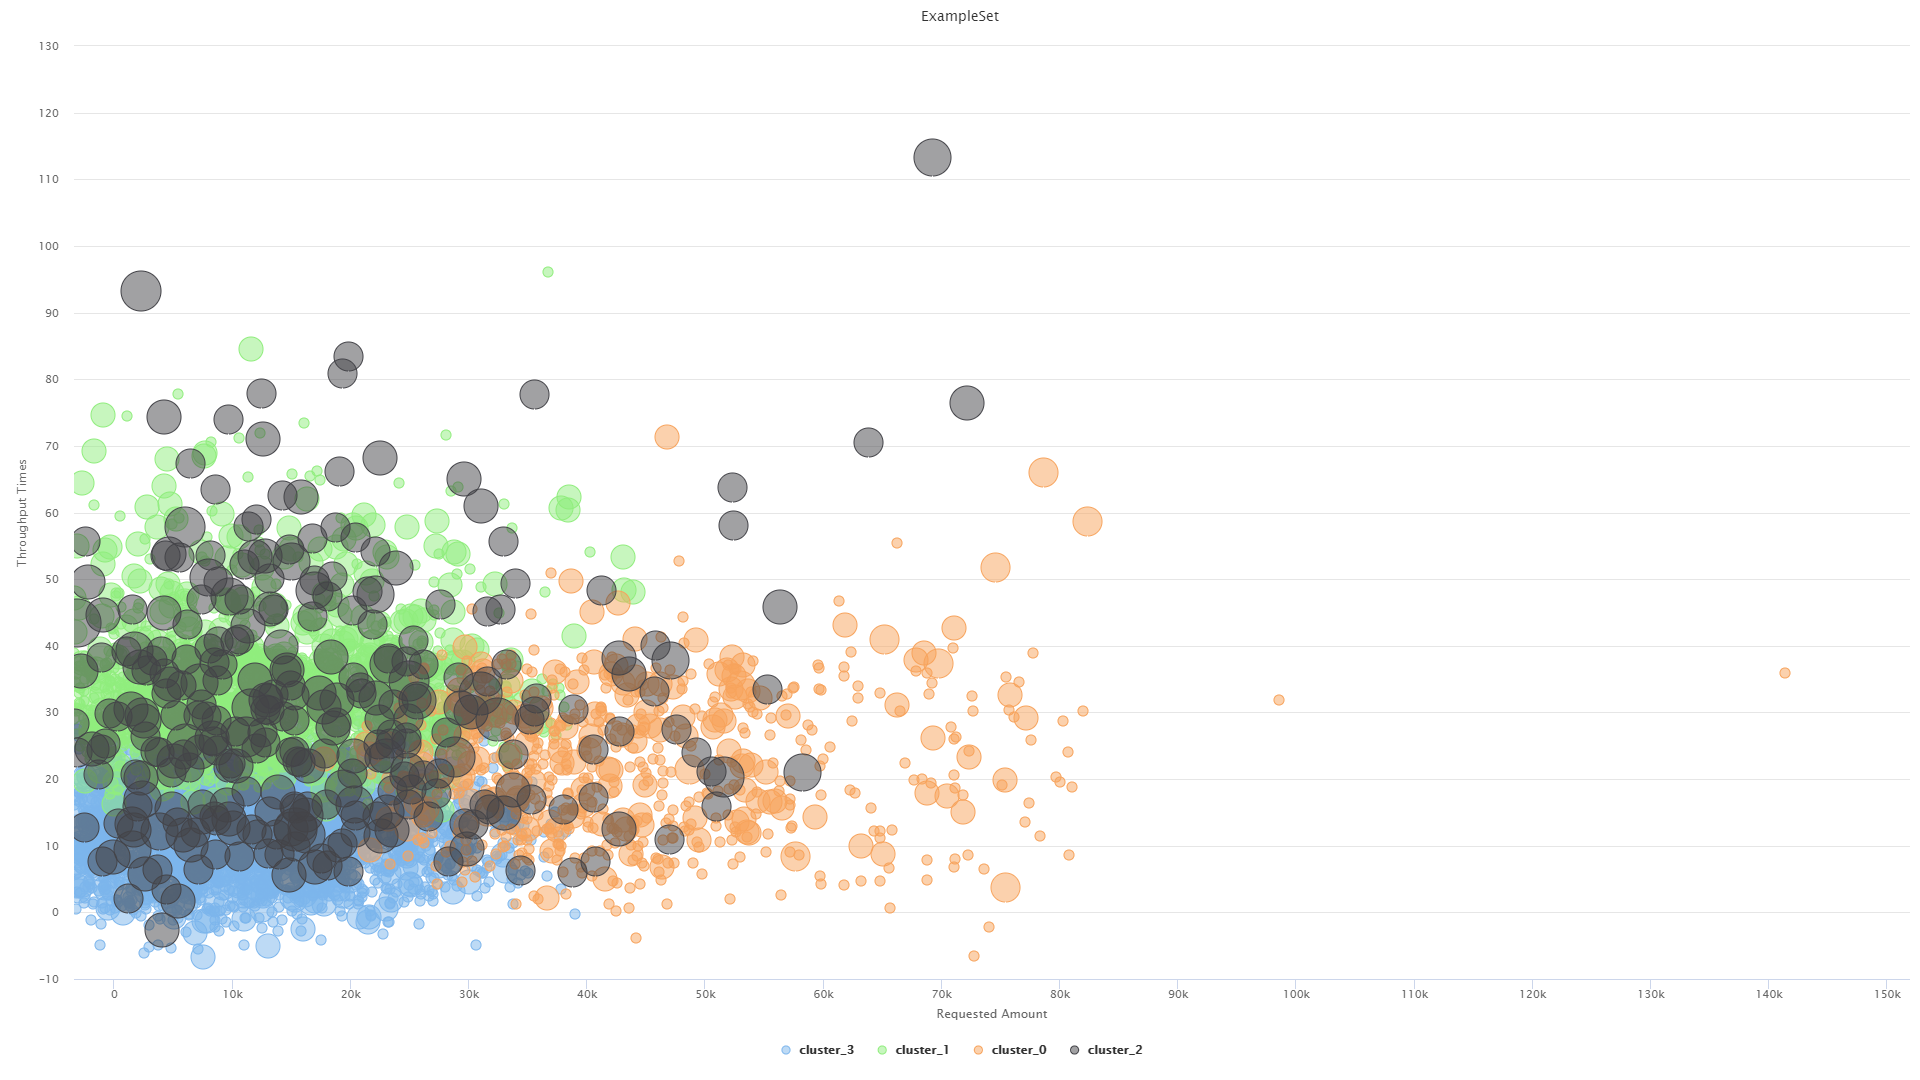
\includegraphics[width=\textwidth]{img/QUESTION_3a_kmeans_4_offers_amount.png}
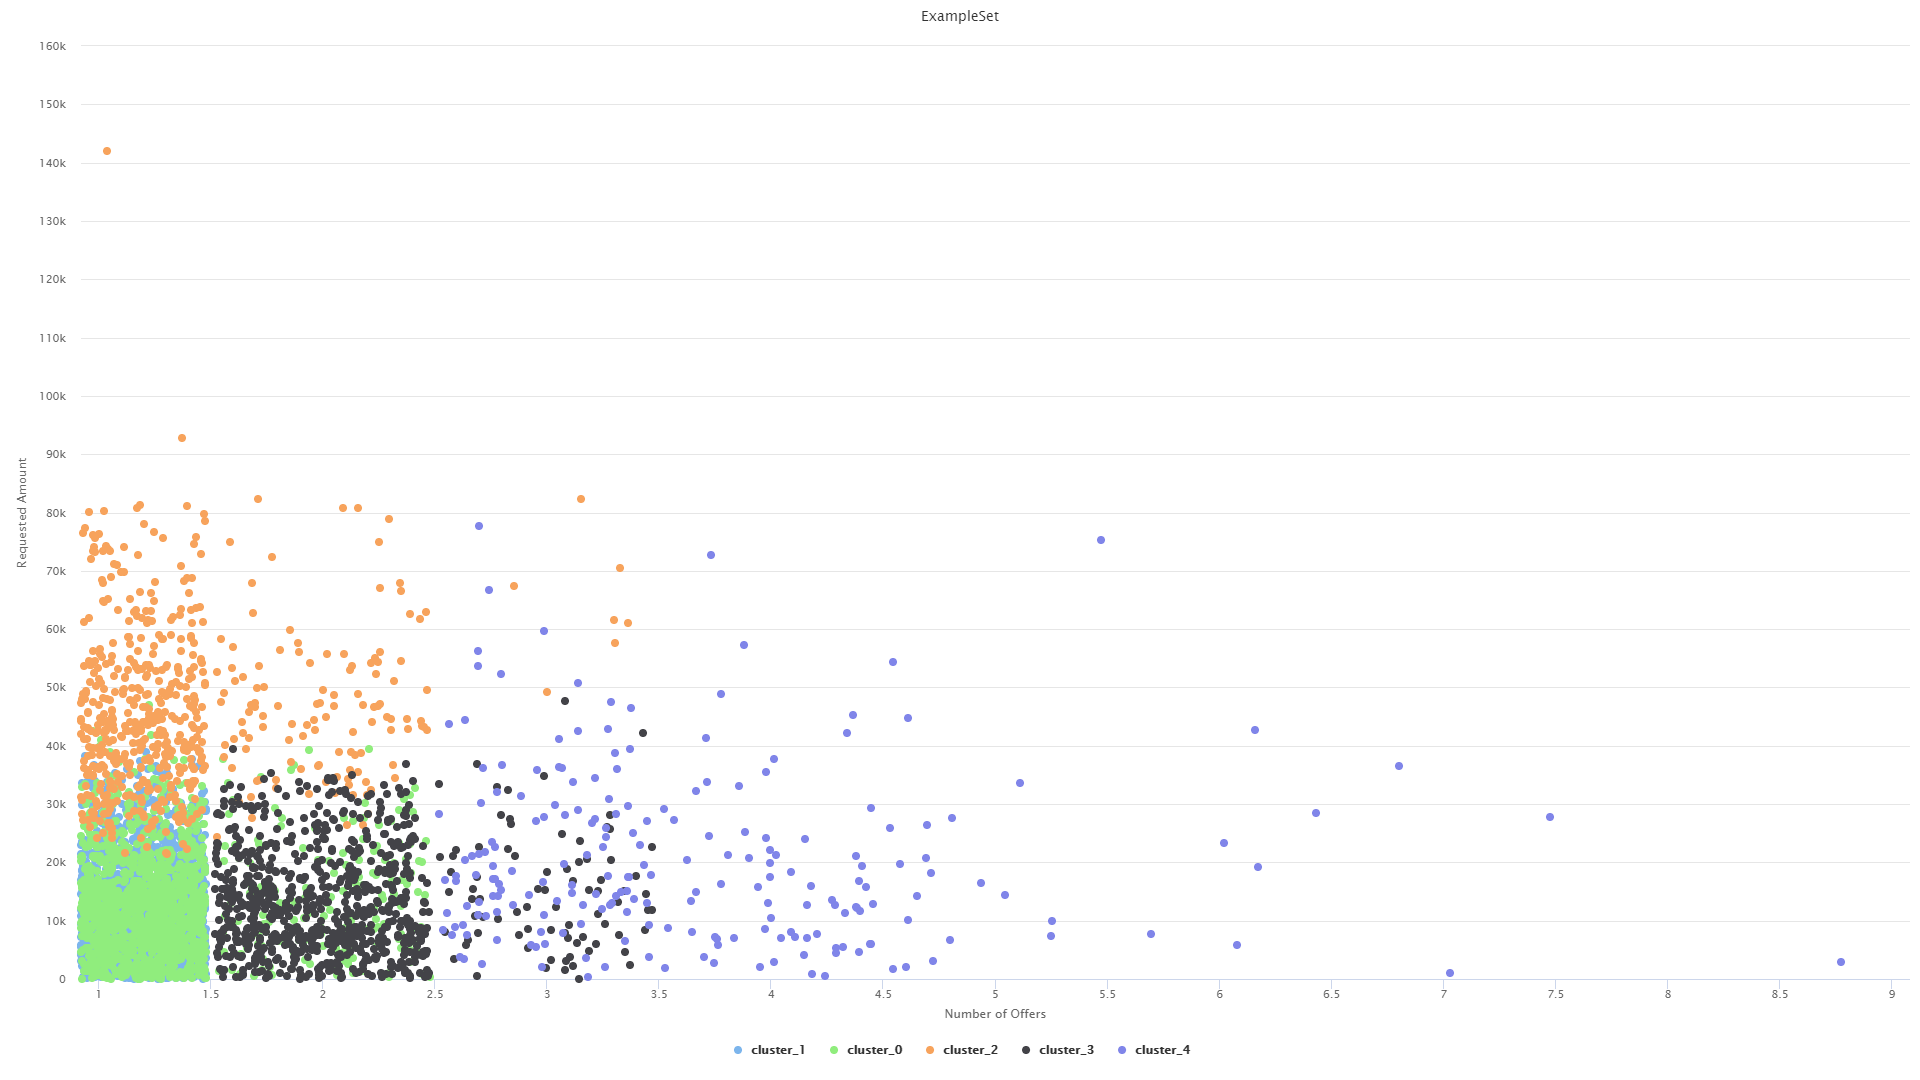
\includegraphics[width=\textwidth]{img/QUESTION_3a_kmeans_5_offers_amount.png}

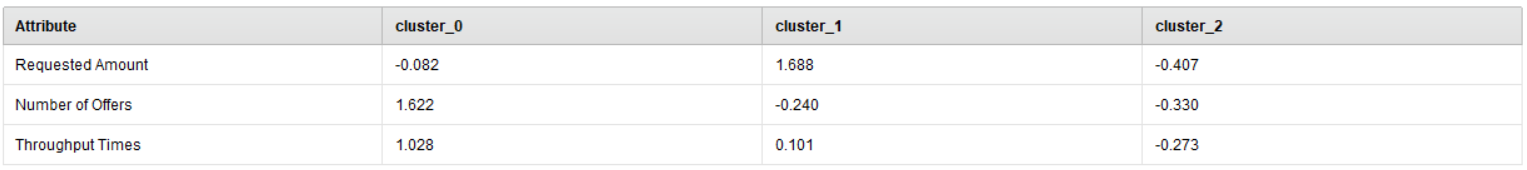
\includegraphics[width=\textwidth]{img/QUESTION_3a_kmeans_3_centroids.png}
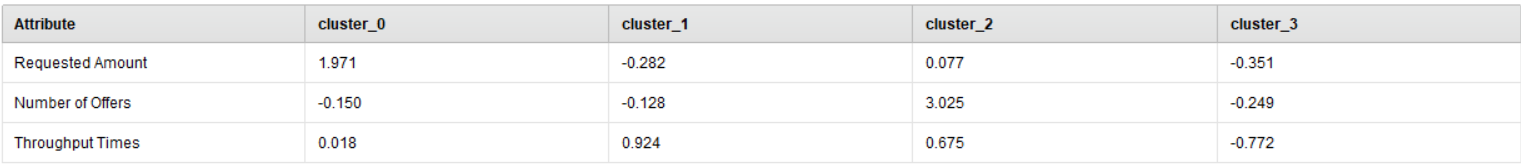
\includegraphics[width=\textwidth]{img/QUESTION_3a_kmeans_4_centroids.png}
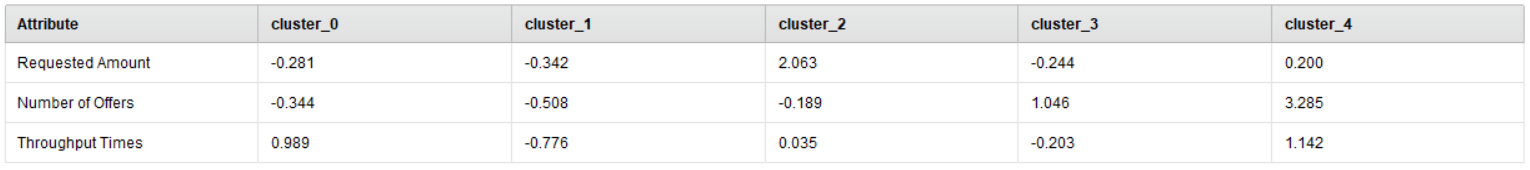
\includegraphics[width=\textwidth]{img/QUESTION_3a_kmeans_5_centroids.png}

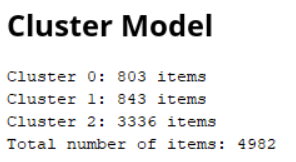
\includegraphics[width=\textwidth/3]{img/QUESTION_3a_kmeans_3_cluster_sizes.png}
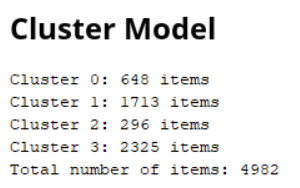
\includegraphics[width=\textwidth/3]{img/QUESTION_3a_kmeans_4_cluster_sizes.png}
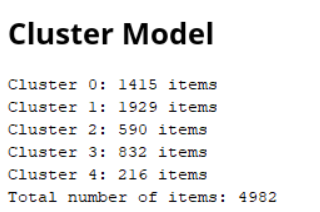
\includegraphics[width=\textwidth/3]{img/QUESTION_3a_kmeans_5_cluster_sizes.png}

\subsection*{(b)}


\end{document}